\chapter{Applying the PSO to the FAP}
\section{Introduction}
Particle Swarm Optimization (PSO) as discussed in the overview (see page \pageref{sec:PSO}) is an algorithm that is largely based on the flying behaviour exhibited by a flock of flying birds. Which is why the core
of the algorithm is based upon vector math, with new positions and velocities being calculated after each iteration of the algorithm. Thus, each particle position, is represented by a D-dimensional vector and
is then simulated flying through the D-dimensional space using the velocity equation (see \pageref{}).

The performance of the Global PSO is benchmarked and outline in the previous chapter. Most of the problems to which PSO has been applied to, to date have been problems where the position of particles have a 
constant D-dimensional space, which is to formally state \emph{the dimensionality of a particle position in its entirety, is constant}.

This constant dimensionality introduces a intriguing problem if you want to apply the PSO to an inherent multi-dimension problem like the Frequency Assignment Problem (FAP). In this chapter we will provide
a discussion on how, we the authors, went about in applying the PSO to the FAP.

We will start of by first explaining what we deemed as a position for a particle in the Frequency Planning domain. This definition of the particle position is important because it plays a central part in
how we "fly" our particles through the Frequency planning domain. After the position definition, we will define how each position will be evaluated and formally define the fitness function our swarm will use.

Arguably the most important part of the swarm, is how we calculate the velocity of a particle and moving it to a new position in the search space. A discussion on the velocity function we have 
developed will be discussed in the section after the fitness function.

After the velocity function section we will discuss a new mechanism for selecting the global best which allowed us to get better fitness values and therefore direct the swarm more. Finally we will end this section
of with a section on the how the swarm utilizes history to produce better results.
\section{A Position in the Frequency Planning domain}
In this section we will describe what a position is in the Frequency Planning domain. We will start of by first describing what a Frequency Plan is as well as provide the general structure to represent such a plan.
We will also describe some of the hard and soft constraints and how it molds the plan to be suitable for a network.

A Frequency plan, is almost exactly as the name implies. A plan that outlines frequency usage for a wireless network. The benchmark problems we will be using all pertain to cellular phone networks. For Cellular networks,
the frequency plan outlines what frequency must be allocated to what transceiver. With this basic definition, the problem seems relatively trivial to solve if one assumes that one either has a infinite number of frequencies
or the amount of frequencies available to our disposal is more than the amount of transceivers in the network. 

The reality is, that there are only a finite amount of frequencies available for cellphone transmissions. Hence a regulatory body needs to assign frequencies to cellphone network operators for use in their networks. A regulatory
body is needed because, if a network operator just uses any frequency it wants, it is bound to interfere with someone else also utilising the frequency.

The assigned frequencies are also not a huge portion of the entire spectrum. If we look at one of our benchmark problems, Siemens1, the alloted spectrum is from frequency 16 to frequency 90. Which gives the network operator 74
frequencies to use in its network without considering other constraints. 

Besides the Electro-magnetic constraints that are also applicable here, there are regulatory constraints, like for instance frequencies in the spectrum that are by no means allowed to be used. These frequencies are referred to as
globally blocked frequencies and are hard constraints. There are also locally blocked frequencies, which apply only in certain regions of the geographical landscape of the network.

As discussed in chapter 2 (page \pageref{chpt:celltech}) and 3 (see page \pageref{chpt:fap}). A Cellphone network is divided into a number of cells, and each cell requires a certain number of transceivers to service its corresponding
area. This number of transceivers is based on the expected volume of traffic that a particular cell will experience at peak network usage. Due to this variability in the expected amount of traffic a cell is supposed to handle, the nature
of the frequency assignment problem is of a multi dimensional nature.
~
~
\begin{figure}[ht]
	\centering
	\setlength \fboxsep{0pt}
	\setlength \fboxrule{0.5pt}
	\fbox{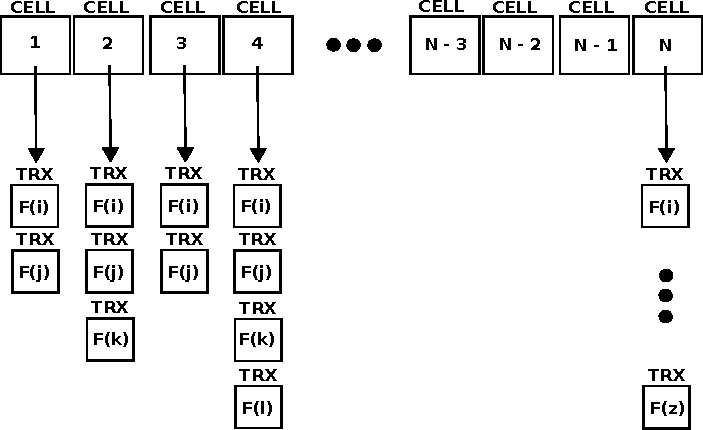
\includegraphics[width=4.8in, height=3.5in]{./pictures/fapPlanDiagram.pdf}}
	\caption{The Structure of a Frequency Plan}
	\label{fig:fapPlan}
\end{figure}
~
As can be seen in figure \ref{fig:fapPlan} a cellular network can have any amount ($N$ in the figure) of cells to attain the desired coverage over the geographical landscape. In our benchmarks problems the cellular networks have a number of
cells ranging from 500 to 1000+. The most important part of the plan, is the actual TRX's within each cell. In the figure we can clearly see, how the amount of TRX's vary from one cell to the next. $F(i)$ is a frequency at position $i$ from
the available usable spectrum. 

Note based on the structure of the plan depicted in figure \ref{fig:fapPlan} there is no concept of which cell interferes with which other cell and if their is indeed interference, how much is inferred as a result. All this information isn't part
of the plan. Instead this information, for purpose of this dissertation is supplied by the benchmark. 

This information is referred to as the interference matrix. Within this interference matrix each entry references two cells entries Cell A and Cell B. The entry then lists the amount of interference that occurs when Cell B interferes with 
Cell A\footnote{Interference occurs based on the electromagnetic constraints as defined in chapter 3}.

A Frequency Plan is a possible solution to the Frequency Assignment Problem. Therefore in the PSO, we the authors have developed, each Particle's position in the solution space is represented by a frequency plan. As mentioned earlier, moving particles through the frequency plan solution space introduces an interesting problem due to the multi-dimensionality of a plan. We will describe how particles are moved from one position to another through the solution space in section \ref{sec:velocityFAP}

In this section we have given a description of what a our PSO will use a position in the frequency planning domain. We outlined the general structure of what a frequency plan is as well as defined how the interference values are retrieved when
two cells interfere. In the next section we will define the fitness function that our PSO's uses. 
\section{The Fitness Function}
In this section we will provide a discussion on the fitness function we utilise in all the variants of our swarms to rate each individual particle position of the swarm.

As discussed in the previous section, the set of benchmark problems we apply our particle swarms to define the amount of interference incurred when two cells assigned frequencies interfere. This interference information is referred to as 
the interference matrix. Each pair of cells has two interference values defined, The first value referred to as Co-channel interference is when the frequency of one TRX is the equal to a TRX in the other cell. The second value, called 
adjacent channel interference is when the frequency of a TRX in one cell differs by 1 with another TRX from the other cell.

Evaluation of a frequency plan to determine its fitness value is a simple process. The evaluation procedure goes through each pair of cells defined in the interference matrix where it looks up both cells in the frequency plan. The second
cell is said to interfere with the first cell. Therefore each TRX in the first cell is checked with all the TRX's of the other cell. Depending on whether how the frequencies differ from each other, the fitness procedure adds either the
co-channel or the adjacent channel interference to a summing variable. This procedure is mathematically defined in chapter 3 see page \pageref{E:costFunction} for the formal equation. 

With regard to our benchmarks, not all interference values are added to the summing variable, since each of the benchmarks define a Minimum Tolerable interference variable. Which means that if a given interference value is either equal or
less than this defined value it is acceptable and won't have a impact on the overall plan.

In this section we outlined the basic fitness function our PSO will use to rate the feasibility of particles after each itertation. In the next section we will define how the particle move from one iteration to the next in the solution space.

\section{Velocity Function for Frequency Planning}
\label{sec:velocityFAP}
The Velocity function is arguably the core of the PSO algorithm. It is the procedure by which particles in the swarm move from one point to another point in the solution space. 

The velocity function doesn't blindly move a particle from one point to another but instead, it takes the particle history into account as well as the best particle in the swarm. Therefore, the velocity function is the core means by which
the swarm explores the solution space. A more thorough explanation is provided on page~\pageref{sec:particleVelocity}.

In this section we will provide a discussion on the process we the authors went through to develop a velocity function that is suitable for particles to move from one Frequency plan to another. We will start of explaining our first and worst
method. With each method we define we will give an outline of the problems associated with it. We will end of this section with our primary method which has obtained the best results.

\subsection{Movement in the Frequency Planning domain}
The standard velocity equation works on the basis of vector math. Each particle has a velocity and position which is represented by a standard mathematical vector. The standard equation basically just alters the direction the particle is moving
to move to a more promising position in the solution space.

Vector math has standard basic operations defined for adding,subtracting and multiplication. Hence, applying the PSO to problems that are either mathematical functions or problems that map well to the vector domain is a straight forward trivial process.
With regard to the Frequency planning domain an important question needs to be answered. How to move one multi dimension frequency plan to another ?

We the authors answered the question by thinking of the frequency plan and its dimensionality in a different manner. The most important realization is that, we don't have to develop a procedure that moves a whole plan to another taking into the account
the dimensionality etc. Rather, we opted to disregard the plan as a whole and just apply the velocity function at a much smaller scale. Thus, the velocity function is applied at the lowest level of a frequency plan.

The basic idea about our velocity function is for the movement of the swarm to be at a much finer granularity. Therefore, when a particle needs to move towards a global best particle, the velocity procedure goes into the intricate details of the particle wanting to move and the global best particle. Hence, the procedure goes into each cell defined in the frequency plan represented by the standard particle as well as the global best particle.

For each cell in the frequency plan, the standard PSO equation with inertia is applied to the TRX value. Thus each TRX value is moved in the general direction (on the frequency domain) towards the TRX value defined in the same cell of the global best frequency plan.

The velocity function we the authors have developed is therefore simplified from being a procedure that needs to move around in a multidimensional space, to move values in a 1 dimensional space. Therefore, our velocity function retains the simplicity of the original PSO algorithm as well as the general concept it is based upon.

\subsection{Keeping frequencies bounded}
We the authors, have defined the basic concept that we will use in our swarm to allow the individual particles to move around in the frequency domain. But this alone is not enough, since the swarm currently has no concept of the constraints that exist in the domain. These constraints include what frequencies are
allowed to be used and which must be avoided. Therefore, the velocity function needs to be altered to make the swarm in some sense aware, and hence keep the particle positions bounded within the allowable search space. 

The boundary check we implemented was fairly trivial. The check only applied when one of the following conditions were met after the calculated velocity was applied to the current position:
\begin{itemize}
\item If a TRX frequency is above the maximum allowable frequency (higher bound) given to the network. 
\item If a TRX frequency is below the minimum allowable frequency (lower bound) given to the network.
\end{itemize}
A mod operation is applied to the value to bring it within the allowable range. If for instance, the maximum allowable frequency is 50, and the TRX value (after velocity) is 56. The 56 value gets modded with 50 to produce a value of 6. This modded value is then
added to the minimum allowable frequency. In essence, the value is wrapped around to always be within acceptable range. 

The not so trivial case is when the frequency value is lower that the minimum frequency given to the network. This is because modding the frequency value has no effect. For example, if the lowest allowable frequency is 20 and the TRX value after movement is 15.
Modding the TRX value of 15 with 20 has no effect. Therefore we have opted for the following methods to solve this problem:

\begin{enumerate}
\item First subtract the lower value from the minimum allowable frequency. Then add the result to the minimum allowable frequency. The resultant value is checked again whether it oversteps the bounds of the maximum allowable frequency and bounded accordingly.
\item Add the lower value to the minimum allowable frequency. The resultant value is checked whether it oversteps the bounds of the maximum allowable frequency and bounded accordingly.
\item Repeatedly subtract the lower value from the maximum allowable frequency until the resultant frequency is within the acceptable frequency range.
\end{enumerate}

An important notion to consider is that based on the velocity equation it is entirely in the realm of possibility that a TRX value after movement might contain a negative value. Our boundary check solves this problem by first taking the absolute value of negative TRX value. The boundary check then treats the now positive TRX value, as a normal value that needs to be bounded.

\subsection{Using indices instead of frequencies}
In the first iteration of our velocity equation the swarm worked with raw frequency values. But upon closer inspection and the frequency range the swarm was using to move around we noticed that the swarm wasn't prohibited from using Globally Blocked Channels or Locally Blocked Channels. Hence, the swarm increasingly moved towards allocating these prohibited values to TRX's since the fitness function doesn't penalize the use of these frequency values. This is due in part because these values are under no circumstances allowed to be used and thus the fitness function isn't designed to check for these values.

To solve this problem, we the authors proposed two solutions:
\begin{enumerate}
\item Modify the fitness function to penalize a frequency plan if it uses any Globally Blocked Channels or Locally Blocked Channels.
\item Instead of letting the swarm work with raw frequency values, rather let the swarm work with array indices. These array indices indicate positions in a array that has been pre-filled with only \emph{valid} frequencies. Thus the swarm then moves around in a range from 0 to $F$, where $F$ is the size of the array.
\end{enumerate}

With the first solution, the fitness function will have to be modified to levy a penalty if a prohibited frequency value is used. The first proposed solution was disregarded because it introduces complexity which can be completely avoided with the second proposed solution.

Where as with the second solution the fitness function will not have to be modified and the boundary check is simplified since there is no need to check for a lower bound anymore. The boundary check only now has to check for negative index values and if the higher bound is violated which is now, the size of the array.

\section{Building a Global Best}
Selection of the global best particle by the swarm is a very important procedure. After the swarm has determined which particle has achieved the best position, the swarm enters the velocity function phase. 

As discussed in the velocity function section and in the Particle Velocity section on page ~\pageref{sec:particleVelocity} each particle position is then modified to move in the general direction of the global best and personal best position. Therefore the global best acts as a beacon for the rest of the swarm in the solution space to indicate where good solutions seem to be for the rest of the swarm.

Initially the method we the authors used for selecting the global best in our PSO for the FAP didn't not differ at all from the traditional global PSO algorithm. The Swarm would loop through all the particle and apply the fitness function to determine the fitness of the particles position. The algorithm would then iterate over the swarm to determine which particle has the lowest fitness or in Frequency Planning terms or in Frequency planning terms, which plan has the lowest interference overall. The particle with the lowest fitness would then be the global best for that iteration.

Selecting the global best by evaluating the position as a whole seems to be a natural fit. But if we were to analyse a frequency plan in more detail; specifically how a single value in a resident TRX of a particular cell can affect the interference generated by the whole cell. One can come to the conclusion that it is entirely in the realm of possibility that, one bad value in a TRX can overshadow a potential good value of a neighboring TRX similarly the total interference of a cell can overshadow a cell that had very low interference. 

Therefore, in the traditional method of selecting the global best, a particle is actually selected because it contains less overshadowing TRX's. Hence potential good TRX values get lost.

We the authors went about to rectify this problem by exploiting the information the fitness exposes to us much more thoroughly. The information exposed by the fitness function allows us to see what effects certain values have on the interference of the cell. Therefore, to make better use of this information we developed two methods, each one being more fine grained than the other.

\begin{enumerate}
\item Besides the particle knowing its fitness, we changed the structure of a cell to allow a cell to know the interference it resident TRX's generate.
\item Besides the particle also storing the total fitness, each TRX of a particular cell also stores the interference it has generated.
\end{enumerate}

With both these methods, the global best selection scheme needs to be changed to allow the swarm to take advantage of this newly exposed information. The scheme we the authors implemented to take advantage of the information does not look at a particle position fitness as a whole. Instead, the procedure builds a global best position with this new information. 

The global best building scheme works slightly different for each method. For method 1, the scheme loops through the entire swarm and selects the cell with the lowest interference. It then copy this cell and places it in the global best position at the same position it was found at. For method 2 the scheme follows the same procedure with the only difference being that the scheme now copies a TRX value and places it at the same position in the global best position.

When the swarm executed using this new scheme initially it didn't produce good results. This is largely due to the interference information for a cell in method 1 and for a TRX in method 2 gets reset to 0 after each iteration. Which seems to be correct, but 
in essence what is occurring is that after each iteration the swarm is effectively discarding all information gathered in that iteration. 

To enable to this information to direct the swarm a bit more, we changed the algorithm to not reset the interference values per TRX and per Cell to 0. Instead, the interference values for an iteration is now added to the previous iteration interference values stored by the cell and TRX. This also has the net effect, that bad decisions made by the swarm for a particular particle get progressively worse as the swarm progresses.

We the authors, experimented with reseting the gathered information after a certain number of iterations. But it had no significant impact on the overall solution being produced. In some cases, the swarm moved the much worse solution and wasn't able to improve best particle to the previous best particle levels before the information reset.

With this small change to the structure of cells and TRX's. The swarm produced much better frequency plans that had lower total interference that all previous generated plans. In the next chapter we will present these results.

In this section we discussed a new method for selecting the global best particle from a swarm of particles. We also outlined the structural changes we had to make to enable to algorithm to use these new structural changes to generate lower frequency plans. Finally we discussed some of the problems encountered and how we the authors went about solving it. In the next section we will discuss how we incorporated the notion of a particle or rather a cell, keeping history of previous TRX's values.

\section{Keeping History}
In the traditional PSO history is retained by using the particle personal best position to direct the next movement of the particle. Other methods such as inertia also allows history to direct the movement of the particle. With regard to our PSO on the FAP, the algorithm we have develop also uses these concepts. But these concepts are not able to effectively exploit the history of a particle since they have no concept of what combinations of frequency values have been previously used in a cell.

In the algorithm we developed, we borrowed the concept of Tabu Lists from the Tabu Search Algorithm. Using Tabu lists a particle will be able to better exploit the solution space it currently finds itself in. In our algorithm, we incorporated Tabu Lists by adding to each cell a list which keeps track of resident TRX values in the cell for 20 iterations.

Care must be taken to select a max size of the Tabu List since one wants to keep enough history so that the search space can be adequately exploited. The Max Tabu List size must be less than the amount of available frequencies. Finally the max Tabu List cannot be too large, since the amount of checks the algorithm has to do to see if a value is Tabu is a very expensive operation. The operation is expensive, since for each potential value the Tabu List needs to be iterated through to see if the value is Tabu.

Only after the newly calculated velocity has been applied to the current position of a particular particle is the position checked for \emph{collisions}. We say a collision occurs once a value is found to be in the Tabu List. To resolve a collision, we simply randomly select a new valid value which is just a index to a valid frequency value. This randomly selected value is then also checked if it collides with another value in the Tabu List. 

Generation of randomly values continues until a counter variable reaches a value of 50 or any other predefined value. The collision resolving procedure then just simply accepts the last generated value as valid. The reason for the counter variable is because since no track is kept on previously generated values, the collision resolving procedure might indefinitely keep generating values all of them colliding with values presently in the Tabu List.

By incorporating Tabu Lists and the collision resolving procedure, the efficiency of the algorithm reduced dramatically. To increase efficiency of the operations in the algorithm, we paralyzed the collision resolving procedure, the velocity function and the sanitation procedures \footnote{The sanitation procedure consist of all the constraint checks}. Therefore, multiple cells are moved simultaneously to towards other corresponding cells.

The paralization of these procedures increased efficiency of the algorithm. We the authors also noticed a slight side effect because of these operations. The randomness of our random number generator decreased. This effect was noticed because we outputed the counter variable in the collision resolver procedure. When the value was being outputted our algorithm produced much better results. 

The reason for this is because outputting the variable inherently introduces a delay and therefore, the random numbers generators in other threads have different seed values. Hence, with a delay in each parallel thread the numbers generated by the random number generator is more distinct. Without the delay, the because the of the parallelization some threads might start of with similar seed values because the current time is used a seed value for our random number generator \footnote{This is the default behaviour of the .Net 4.0 random number generator}.

Keeping the delay in mind and the effect is has on the final result, we introduced a delay in our collision resolving procedure. The reason the particular procedure was selected was because it was where the effect of delay was first noticed. After performing tests with delays of 5 milliseconds (ms), 10 ms, 15, 20 we settled on 20 ms since it was gave just enough time for a reasonably distinction between seed values used by other parallel threads.

In this section we discussed how we used Tabu Lists from Tabu Search to keep history. We discussed the alterations we had to make to the algorithm to incorporate the new feature as well as outlined the necessary procedures needed to effectively exploit the Tabu Lists. Finally we discussed the effects the Tabu Lists had on the performance of the algorithm and how we the authors went about solving it.

\section{Summary}
